%
%  untitled
%
%  Created by Sergio on 2009-03-18.
%  Copyright (c) 2009 __MyCompanyName__. All rights reserved.
\documentclass[]{article}

% Use utf-8 encoding for foreign characters
\usepackage[utf8]{inputenc}
\usepackage[spanish]{babel}

% Setup for fullpage use
\usepackage{fullpage}

% Uncomment some of the following if you use the features
%
% Running Headers and footers
%\usepackage{fancyhdr}

% Multipart figures
%\usepackage{subfigure}

% More symbols
%\usepackage{amsmath}
%\usepackage{amssymb}
%\usepackage{latexsym}

% Surround parts of graphics with box
\usepackage{boxedminipage}

% Package for including code in the document
\usepackage{listings}

% If you want to generate a toc for each chapter (use with book)
\usepackage{minitoc}

% This is now the recommended way for checking for PDFLaTeX:
\usepackage{ifpdf}

%\newif\ifpdf
%\ifx\pdfoutput\undefined
%\pdffalse % we are not running PDFLaTeX
%\else
%\pdfoutput=1 % we are running PDFLaTeX
%\pdftrue
%\fi

\ifpdf
\usepackage[pdftex]{graphicx}
\else
\usepackage{graphicx}
\fi
\title{A LaTeX Article}
\author{ }

\date{\today}

\begin{document}

\ifpdf
\DeclareGraphicsExtensions{.pdf, .jpg, .tif}
\else
\DeclareGraphicsExtensions{.eps, .jpg}
\fi

%\maketitle


%\begin{abstract}
%\end{abstract}
Este documento servirá de guía en la ejecución de la aplicación graficadora de splines que permite
agregar puntos por el usuario mediante el uso de clicks. Se mostrará la forma de compilar el código
escrito en $C++$ que usa las librerías gráficas de $OpenGL$\cite{OPENGL}.\\

\subsection{Compilación}	
Para compilar el código del graficador se necesita tener instalado un compilador de $C/C++$,siendo
uno de los más recomendados el $gcc$\cite{GCC}, y las librerías para gráficos de $OpenGL$\cite{OPENGL}
con $Glut$\cite{GLUT}.\\

\section{OwnSpliner.cc}

El comando de compilación en una Terminal de Linux sería el siguiente:
\[ \verb=$> g++ ownSpliner.cc -lglut -o ownSpliner= \]
\def\mySize{5}
\begin{figure}[h] %  figure placement: here, top, bottom, or page
   \centering
   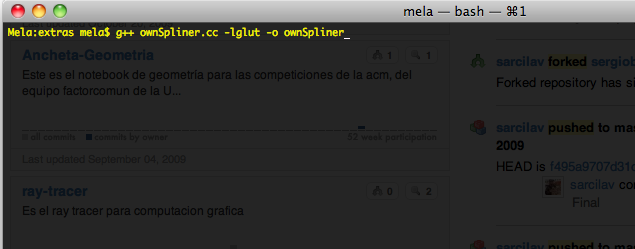
\includegraphics[width=\mySize in]{2.png} 
%   \caption{example caption}
   \label{fig:example}
\end{figure}


\subsection{Ejecución}

Después de tener el ejecutable generado sólo falta ejecutarlo como cualquier otra aplicación por línea de comandos:
\[ \verb=$> ./ownSpliner= \]

\begin{figure}[ht] %  figure placement: here, top, bottom, or page
   \centering
   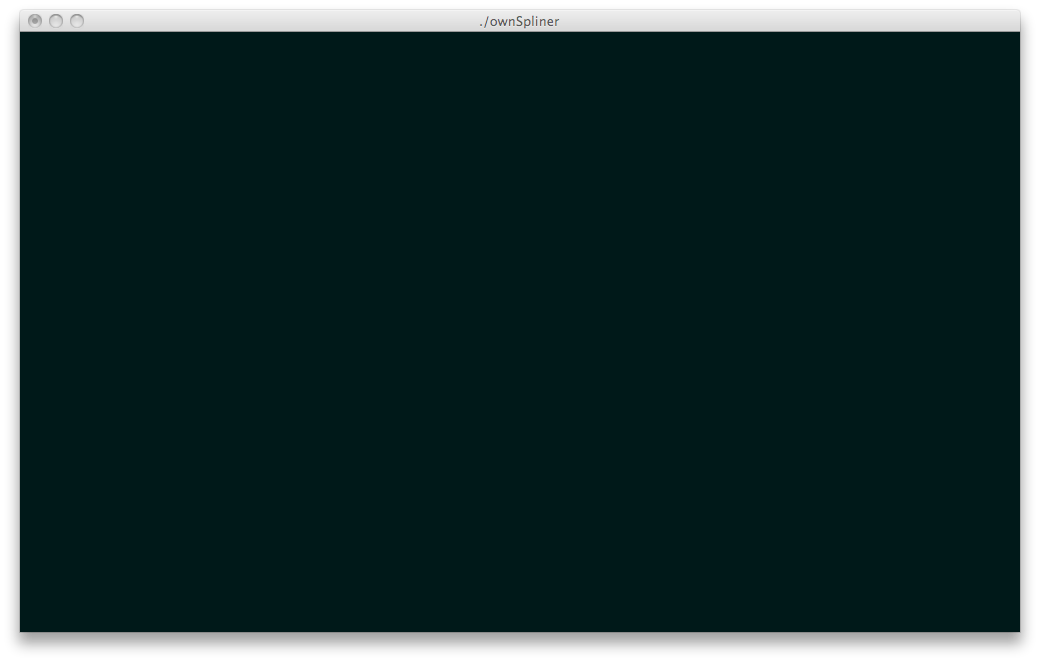
\includegraphics[width=\mySize in]{1.png} 
   \caption{Ventana de la aplicación al abrir}
   \label{fig:example}
\end{figure}

Ahora sólo resta la interacción con la aplicación, el usuario debe crear el primer óvalo con tres puntos
para iniciar el spline cerrado, después de crear los tres puntos el usuario puede crear nuevos puntos 
haciendo click con el mouse.

%\begin{figure}[ht] %  figure placement: here, top, bottom, or page
   \centering
   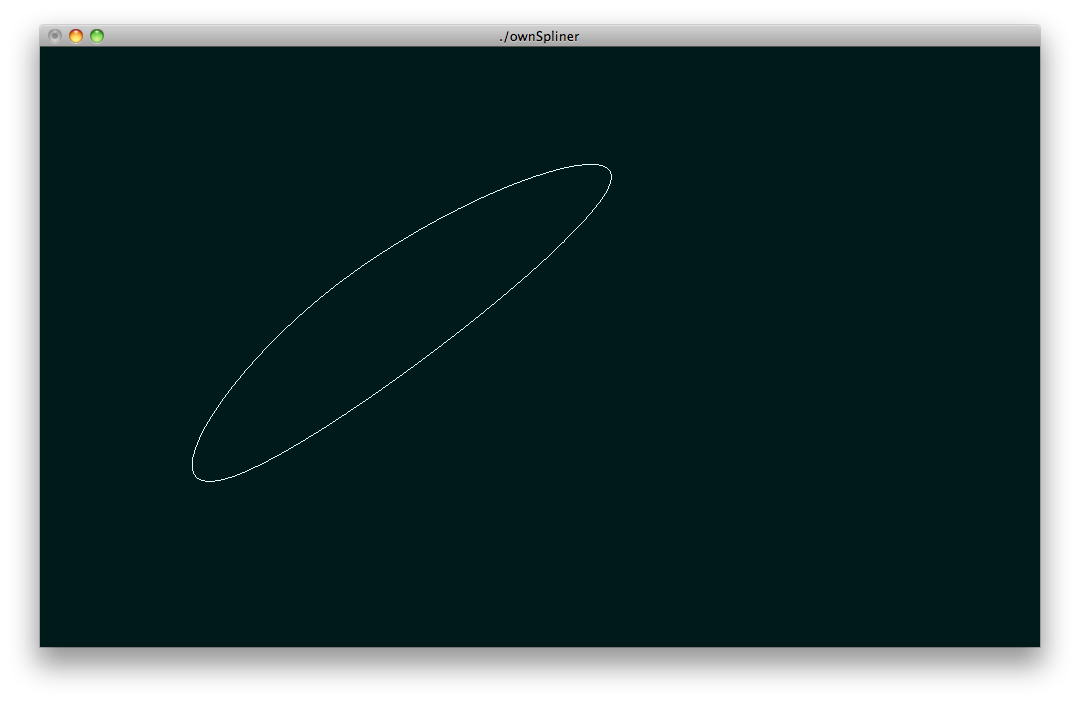
\includegraphics[width=\mySize in]{3.png} \\
Óvalo creado\\
%   \label{fig:example}
%\end{figure}
%\begin{figure}[ht] %  figure placement: here, top, bottom, or page
   \centering
   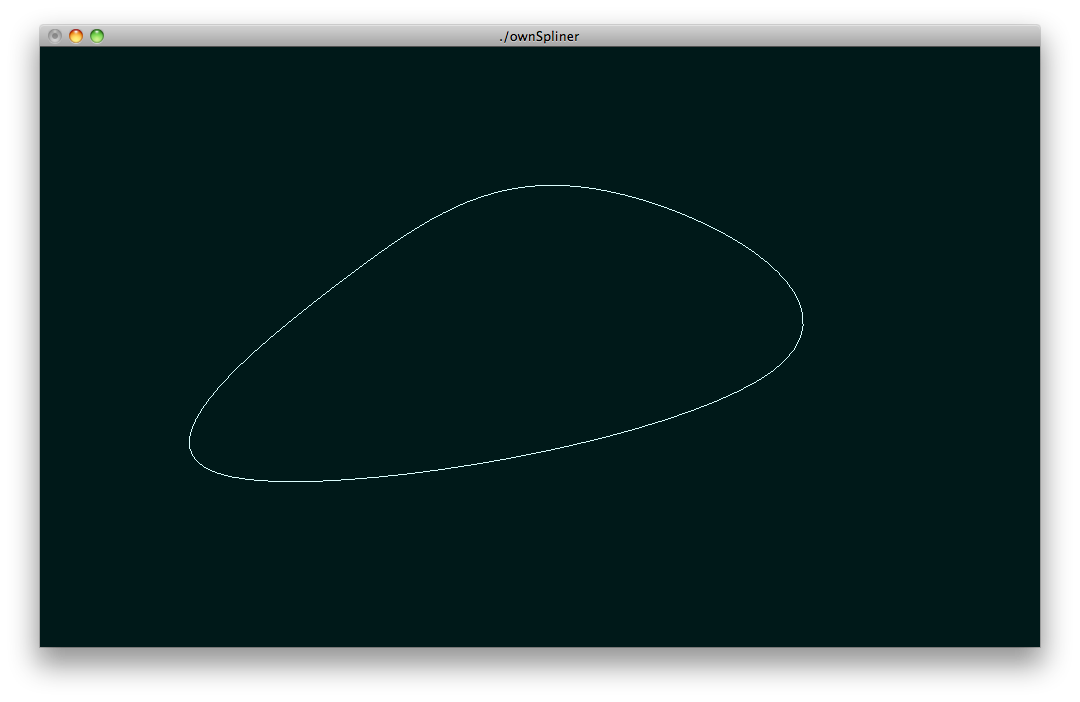
\includegraphics[width=\mySize in]{4.png} \\
Puntos agregados\\
%   \label{fig:example}
%\end{figure}
%\begin{figure}[ht] %  figure placement: here, top, bottom, or page
   \centering
   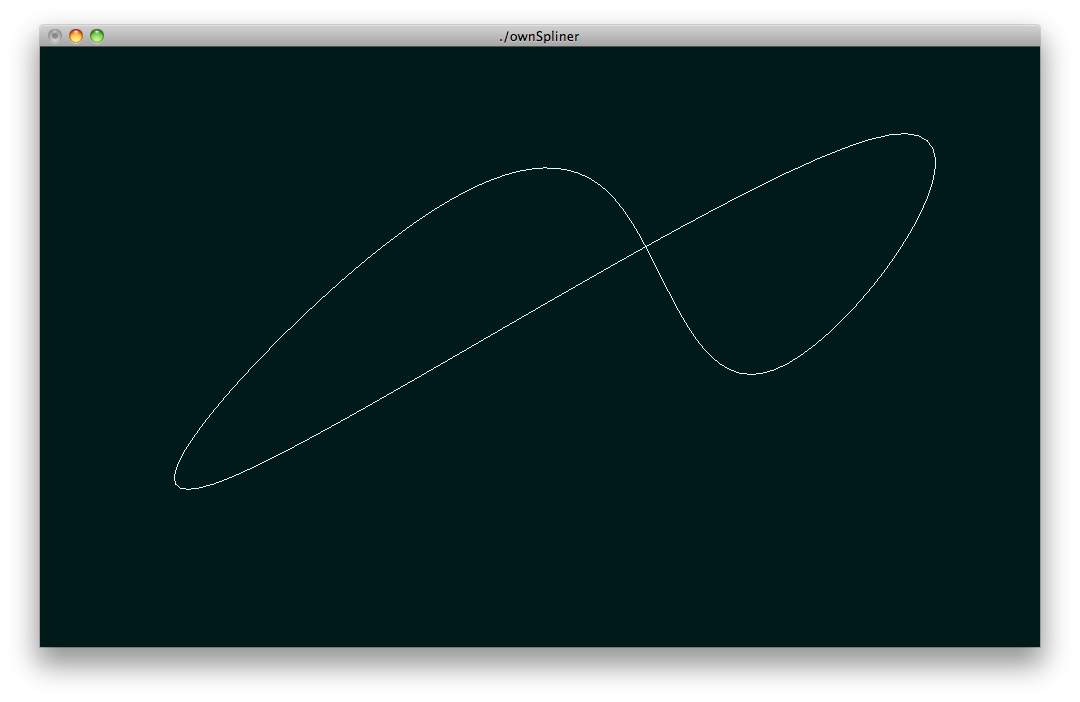
\includegraphics[width=\mySize in]{5.png} \\
   Una figura más elaborada\\
%   \label{fig:example}
%\end{figure}
%\begin{figure}[ht] %  figure placement: here, top, bottom, or page
   \centering
   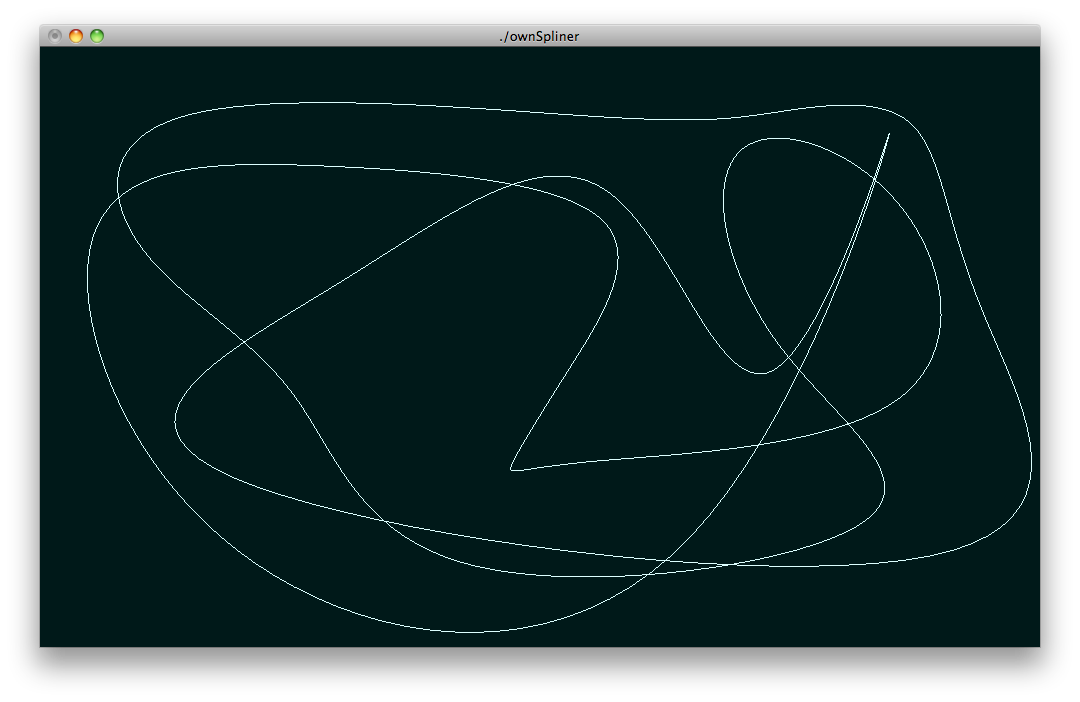
\includegraphics[width=\mySize in]{6.png} \\
   Jugando con más puntos\\
%   \label{fig:example}   
%\end{myGraphs}
\flushleft
En este momento la aplicación no se puede reiniciar, ni borrar la nube de puntos, por lo tanto se debe
volver a la ejecución de la aplicación mediante el comando de Terminal.



\section{linearSpliner.cc}
\subsection{Compilación}	
El comando de compilación en una Terminal de Linux sería el siguiente:
\[ \verb=$> g++ linearSpliner.cc -lglut -o linearSpliner= \]
\def\mySize{5}
%\begin{figure}[h] %  figure placement: here, top, bottom, or page
%   \centering
%   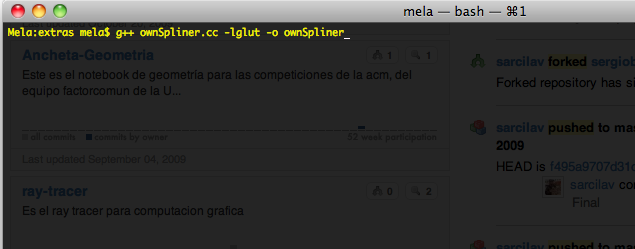
\includegraphics[width=\mySize in]{2.png} 
%%   \caption{example caption}
%   \label{fig:example}
%\end{figure}


\subsection{Ejecución}

Después de tener el ejecutable generado sólo falta ejecutarlo como cualquier otra aplicación por línea de comandos:
\[ \verb=$> ./linearSpliner= \]

\begin{figure}[ht] %  figure placement: here, top, bottom, or page
   \centering
   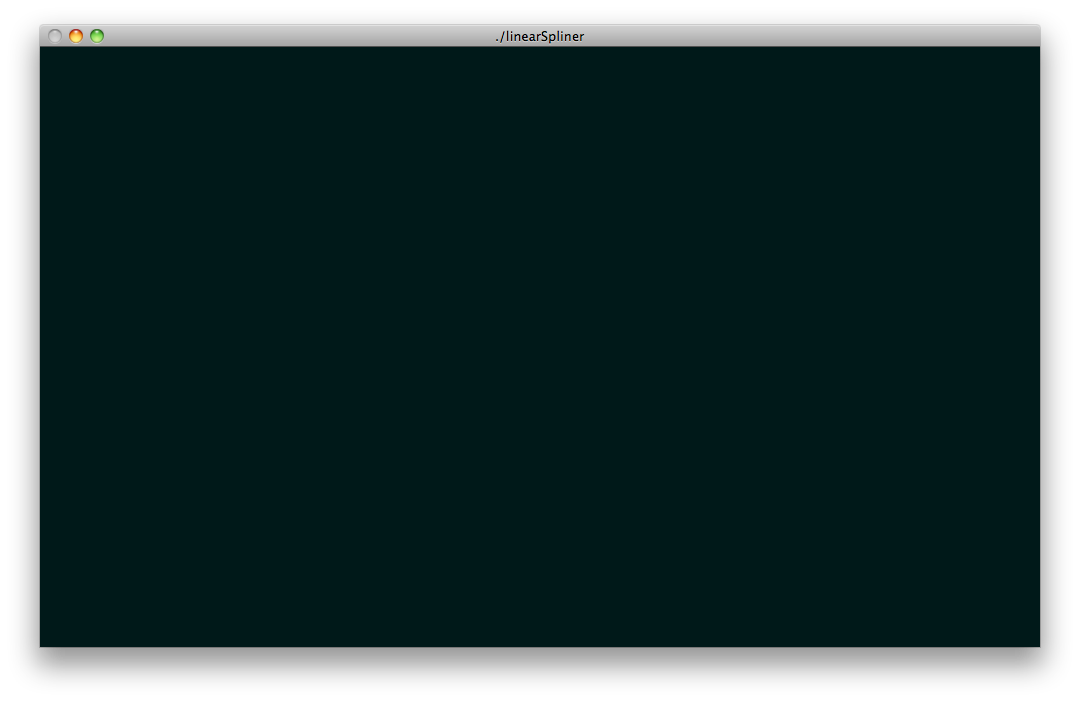
\includegraphics[width=\mySize in]{7.png} 
   \caption{Ventana de la aplicación al abrir}
   \label{fig:example}
\end{figure}

En este momento ya se puede iniciar a crear líneas que se irán uniendo a medida que el usuario hace clicks para
crear nuevos puntos.

%\begin{figure}[ht] %  figure placement: here, top, bottom, or page
   \centering
   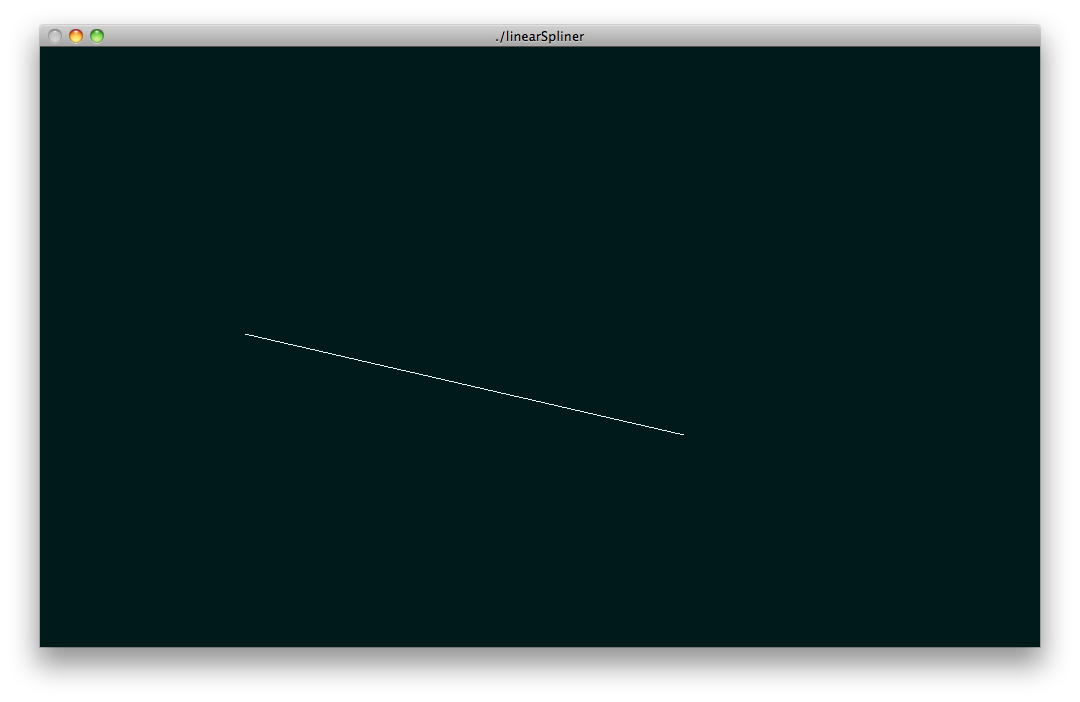
\includegraphics[width=\mySize in]{8.png} \\
Línea\\
%   \label{fig:example}
%\end{figure}
%\begin{figure}[ht] %  figure placement: here, top, bottom, or page
   \centering
   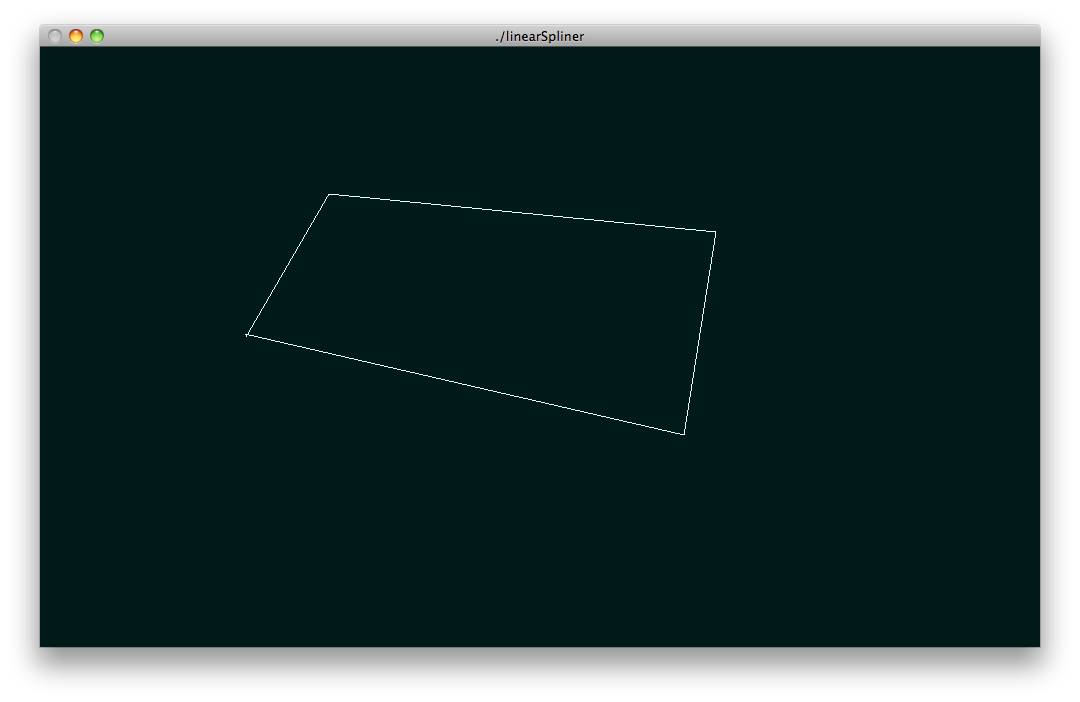
\includegraphics[width=\mySize in]{9.png} \\
Cuadrado\\
%   \label{fig:example}
%\end{figure}
%\begin{figure}[ht] %  figure placement: here, top, bottom, or page
%   \centering
%   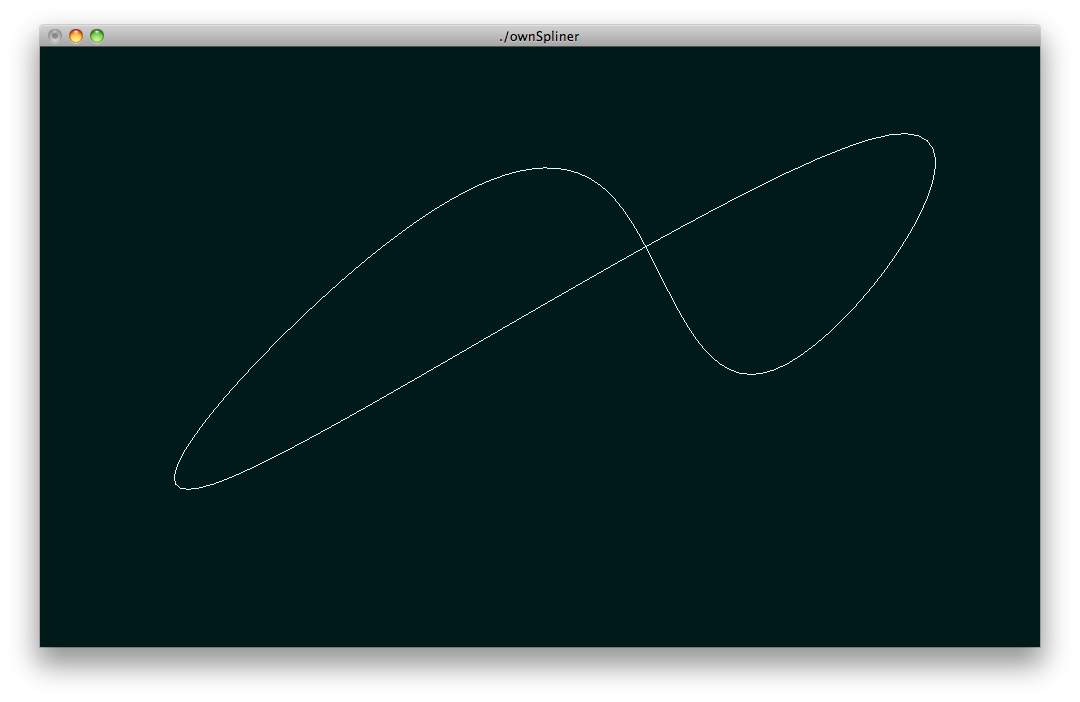
\includegraphics[width=\mySize in]{5.png} \\
%   Una figura más elaborada\\
%%   \label{fig:example}
%%\end{figure}
%%\begin{figure}[ht] %  figure placement: here, top, bottom, or page
%   \centering
%   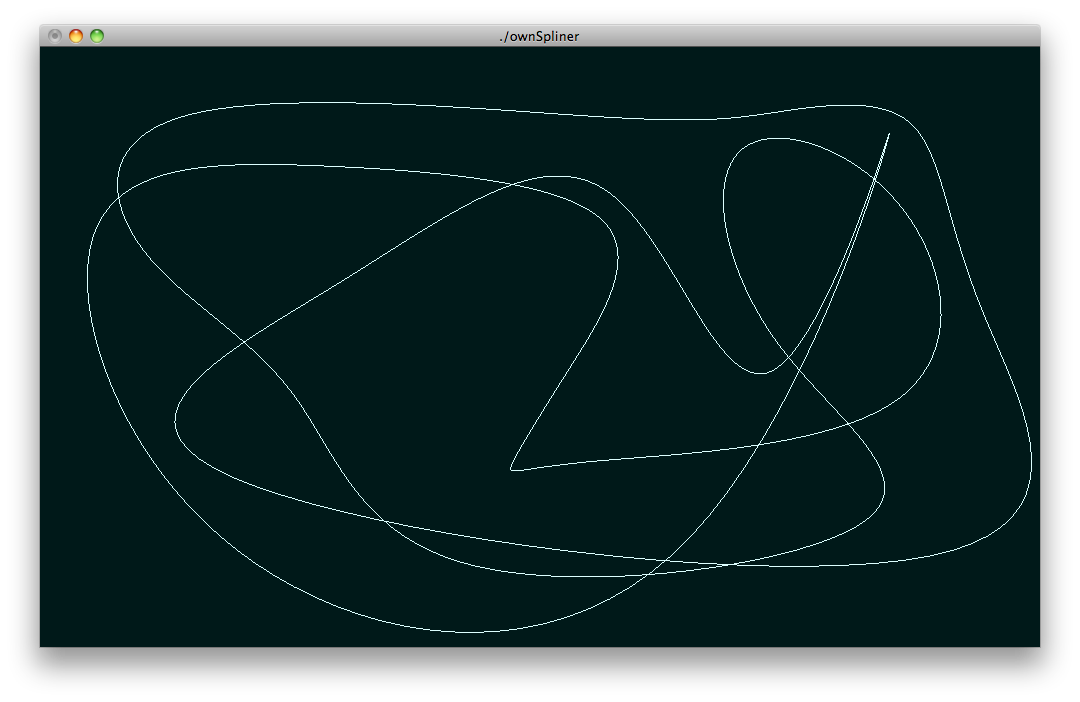
\includegraphics[width=\mySize in]{6.png} \\
%   Jugando con más puntos\\
%%   \label{fig:example}   
%%\end{myGraphs}
\flushleft
En este momento la aplicación no se puede reiniciar, ni borrar la nube de puntos, por lo tanto se debe
volver a la ejecución de la aplicación mediante el comando de Terminal.

\section{splinerStepbyStep.cc}
\subsection{Compilación}	
El comando de compilación en una Terminal de Linux sería el siguiente:
\[ \verb=$> g++ splinerStepbyStep.cc -lglut -o splinerStepbyStep= \]
\def\mySize{5}
%\begin{figure}[h] %  figure placement: here, top, bottom, or page
%   \centering
%   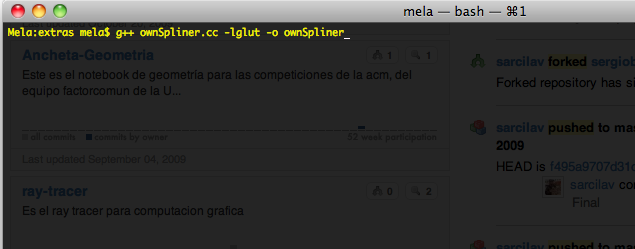
\includegraphics[width=\mySize in]{2.png} 
%%   \caption{example caption}
%   \label{fig:example}
%\end{figure}


\subsection{Ejecución}

Después de tener el ejecutable generado sólo falta ejecutarlo como cualquier otra aplicación por línea de comandos:
\[ \verb=$> ./splinerStepbyStep= \]

\begin{figure}[ht] %  figure placement: here, top, bottom, or page
   \centering
   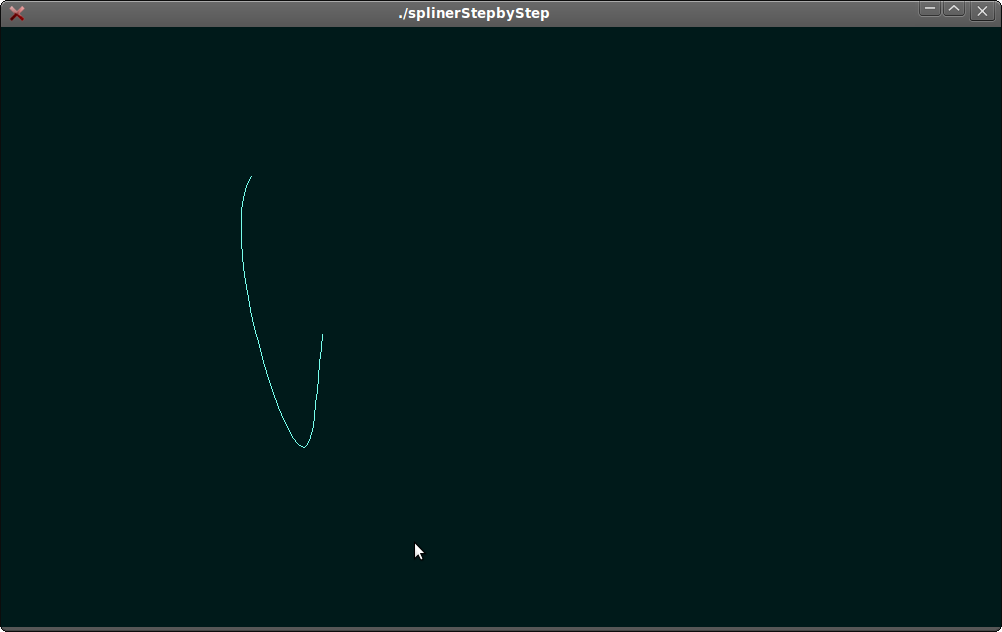
\includegraphics[width=\mySize in]{10.png} 
   \caption{Ventana de la aplicación al abrir}
   \label{fig:example}
\end{figure}

Este graficador no tiene interacción del usuario, lo que se genera es una `animación' de los puntos que se encuentran en el archivo
fuente del programa, para modificar el trazo se deben cambiar los puntos desde el archivo fuente en $C++$, luego se debe
repetir el proceso de compilación y ejecución de la aplicación.

%\begin{figure}[ht] %  figure placement: here, top, bottom, or page
   \centering
   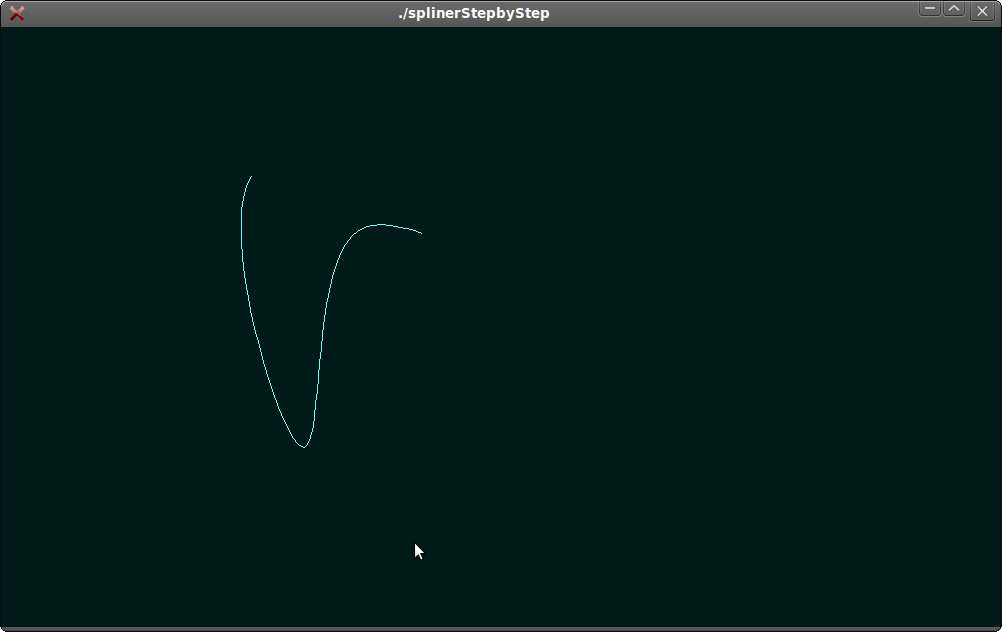
\includegraphics[width=\mySize in]{11.png} \\
%Línea\\
%   \label{fig:example}
%\end{figure}
%\begin{figure}[ht] %  figure placement: here, top, bottom, or page
   \centering
   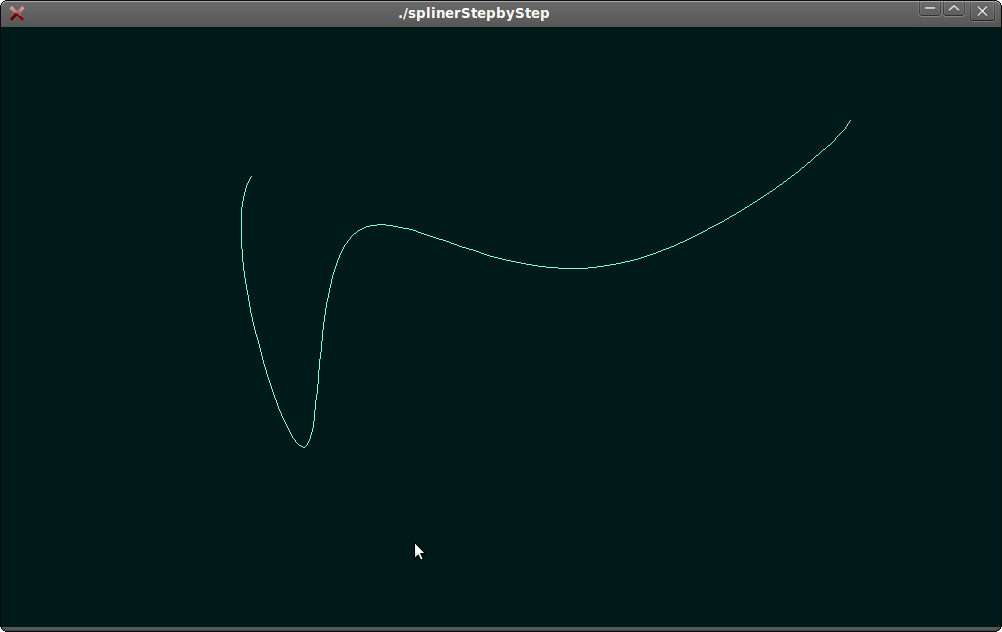
\includegraphics[width=\mySize in]{12.png} \\
%Cuadrado\\
%   \label{fig:example}
%\end{figure}
%\begin{figure}[ht] %  figure placement: here, top, bottom, or page
%   \centering
   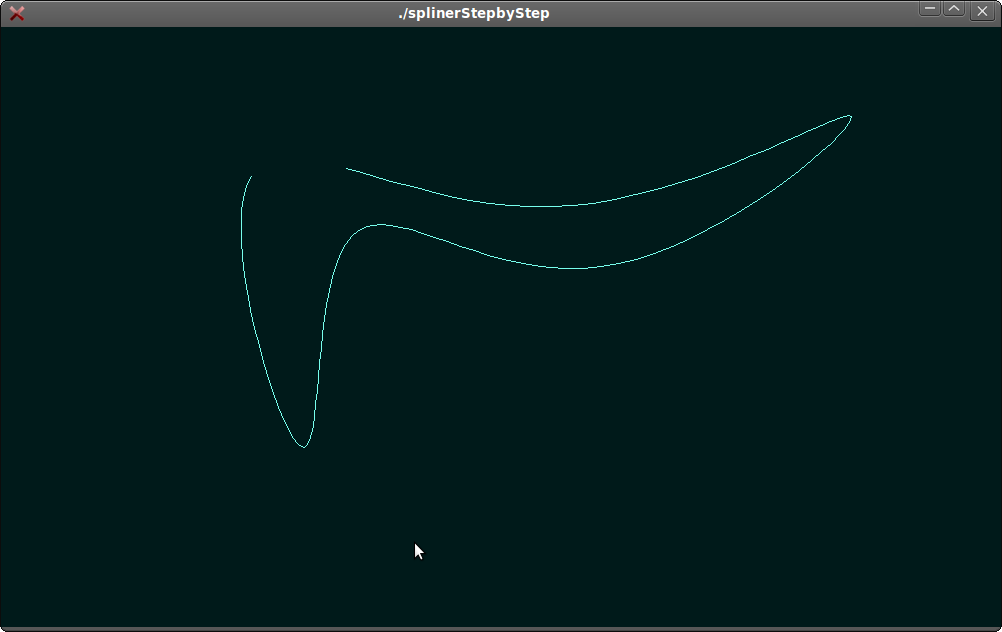
\includegraphics[width=\mySize in]{13.png} \\
%   Una figura más elaborada\\
%%   \label{fig:example}
%%\end{figure}
%%\begin{figure}[ht] %  figure placement: here, top, bottom, or page
%   \centering
%   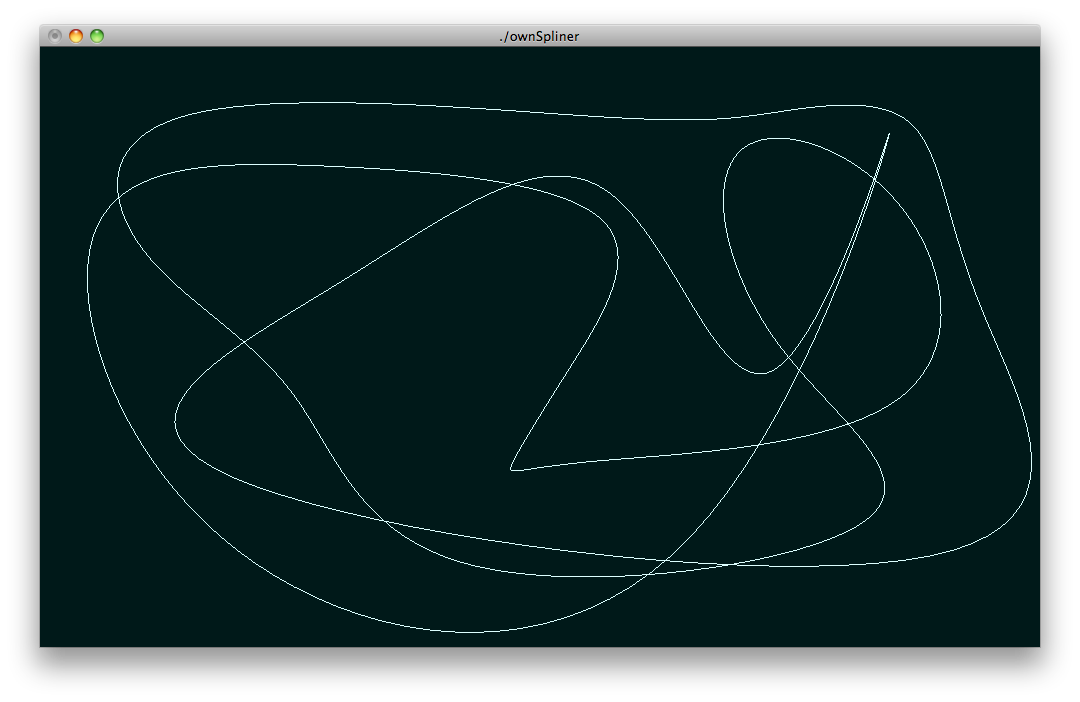
\includegraphics[width=\mySize in]{6.png} \\
%   Jugando con más puntos\\
%%   \label{fig:example}   
%%\end{myGraphs}
\flushleft
En este momento la aplicación no se puede reiniciar, ni borrar la nube de puntos, por lo tanto se debe
volver a la ejecución de la aplicación mediante el comando de Terminal. Esta animación no se detendrá.

\newpage
\begin{thebibliography}{3}
\bibitem{OPENGL} The Industry's Foundation for High Performance Graphics, $http://www.opengl.org$
\bibitem{GCC}  GCC, the GNU Compiler Collection, $http://gcc.gnu.org$
\bibitem{GLUT} OpenGL Utility Toolkit, $http://www.opengl.org/resources/libraries/glut/$
\end{thebibliography}
\end{document}
